\documentclass[journal,12pt,twocolumn]{IEEEtran}

\usepackage{setspace}
\usepackage{gensymb}

\singlespacing


\usepackage[cmex10]{amsmath}

\usepackage{amsthm}

\usepackage{mathrsfs}
\usepackage{txfonts}
\usepackage{stfloats}
\usepackage{bm}
\usepackage{cite}
\usepackage{cases}
\usepackage{subfig}

\usepackage{longtable}
\usepackage{multirow}

\usepackage{enumitem}
\usepackage{mathtools}
\usepackage{steinmetz}
\usepackage{tikz}
\usepackage{circuitikz}
\usepackage{verbatim}
\usepackage{tfrupee}
\usepackage[breaklinks=true]{hyperref}
\usepackage{graphicx}
\usepackage{tkz-euclide}
\usepackage{float}

\usetikzlibrary{calc,math}
\usepackage{listings}
    \usepackage{color}                                            %%
    \usepackage{array}                                            %%
    \usepackage{longtable}                                        %%
    \usepackage{calc}                                             %%
    \usepackage{multirow}                                         %%
    \usepackage{hhline}                                           %%
    \usepackage{ifthen}                                           %%
    \usepackage{lscape}     
\usepackage{multicol}
\usepackage{chngcntr}

\DeclareMathOperator*{\Res}{Res}

\renewcommand\thesection{\arabic{section}}
\renewcommand\thesubsection{\thesection.\arabic{subsection}}
\renewcommand\thesubsubsection{\thesubsection.\arabic{subsubsection}}

\renewcommand\thesectiondis{\arabic{section}}
\renewcommand\thesubsectiondis{\thesectiondis.\arabic{subsection}}
\renewcommand\thesubsubsectiondis{\thesubsectiondis.\arabic{subsubsection}}


\hyphenation{op-tical net-works semi-conduc-tor}
\def\inputGnumericTable{}                                 %%

\lstset{
%language=C,
frame=single, 
breaklines=true,
columns=fullflexible
}
\begin{document}


\newtheorem{theorem}{Theorem}[section]
\newtheorem{problem}{Problem}
\newtheorem{proposition}{Proposition}[section]
\newtheorem{lemma}{Lemma}[section]
\newtheorem{corollary}[theorem]{Corollary}
\newtheorem{example}{Example}[section]
\newtheorem{definition}[problem]{Definition}

\newcommand{\BEQA}{\begin{eqnarray}}
\newcommand{\EEQA}{\end{eqnarray}}
\newcommand{\define}{\stackrel{\triangle}{=}}
\bibliographystyle{IEEEtran}
\providecommand{\mbf}{\mathbf}
\providecommand{\pr}[1]{\ensuremath{\Pr\left(#1\right)}}
\providecommand{\qfunc}[1]{\ensuremath{Q\left(#1\right)}}
\providecommand{\sbrak}[1]{\ensuremath{{}\left[#1\right]}}
\providecommand{\lsbrak}[1]{\ensuremath{{}\left[#1\right.}}
\providecommand{\rsbrak}[1]{\ensuremath{{}\left.#1\right]}}
\providecommand{\brak}[1]{\ensuremath{\left(#1\right)}}
\providecommand{\lbrak}[1]{\ensuremath{\left(#1\right.}}
\providecommand{\rbrak}[1]{\ensuremath{\left.#1\right)}}
\providecommand{\cbrak}[1]{\ensuremath{\left\{#1\right\}}}
\providecommand{\lcbrak}[1]{\ensuremath{\left\{#1\right.}}
\providecommand{\rcbrak}[1]{\ensuremath{\left.#1\right\}}}
\theoremstyle{remark}
\newtheorem{rem}{Remark}
\newcommand{\sgn}{\mathop{\mathrm{sgn}}}
\providecommand{\abs}[1]{\left\vert#1\right\vert}
\providecommand{\res}[1]{\Res\displaylimits_{#1}} 
\providecommand{\norm}[1]{\left\lVert#1\right\rVert}
%\providecommand{\norm}[1]{\lVert#1\rVert}
\providecommand{\mtx}[1]{\mathbf{#1}}
\providecommand{\mean}[1]{E\left[ #1 \right]}
\providecommand{\fourier}{\overset{\mathcal{F}}{ \rightleftharpoons}}
%\providecommand{\hilbert}{\overset{\mathcal{H}}{ \rightleftharpoons}}
\providecommand{\system}{\overset{\mathcal{H}}{ \longleftrightarrow}}
	%\newcommand{\solution}[2]{\textbf{Solution:}{#1}}
\newcommand{\solution}{\noindent \textbf{Solution: }}
\newcommand{\cosec}{\,\text{cosec}\,}
\providecommand{\dec}[2]{\ensuremath{\overset{#1}{\underset{#2}{\gtrless}}}}
\newcommand{\myvec}[1]{\ensuremath{\begin{pmatrix}#1\end{pmatrix}}}
\newcommand{\mydet}[1]{\ensuremath{\begin{vmatrix}#1\end{vmatrix}}}
\numberwithin{equation}{subsection}
\makeatletter
\@addtoreset{figure}{problem}
\makeatother
\let\StandardTheFigure\thefigure
\let\vec\mathbf
\renewcommand{\thefigure}{\theproblem}
\def\putbox#1#2#3{\makebox[0in][l]{\makebox[#1][l]{}\raisebox{\baselineskip}[0in][0in]{\raisebox{#2}[0in][0in]{#3}}}}
     \def\rightbox#1{\makebox[0in][r]{#1}}
     \def\centbox#1{\makebox[0in]{#1}}
     \def\topbox#1{\raisebox{-\baselineskip}[0in][0in]{#1}}
     \def\midbox#1{\raisebox{-0.5\baselineskip}[0in][0in]{#1}}
\vspace{3cm}
\title{Assignment 5}
\author{GAYATHRI S}
\maketitle
\newpage
\bigskip
\renewcommand{\thefigure}{\theenumi}
\renewcommand{\thetable}{\theenumi}
Download all python codes from 
\begin{lstlisting}
https://github.com/Gayathri1729/SRFP/tree/main/Assignment5
\end{lstlisting}
%
and latex-tikz codes from 
%
\begin{lstlisting}
https://github.com/Gayathri1729/SRFP/tree/main/Assignment5
\end{lstlisting}
%
\section{QUADRATIC FORMS-2.64}
A cricket ball is thrown at a speed of 28$ms^{-1}$ in a direction 30$\degree$ above the horizontal.Calculate
\begin{enumerate}
\item[a)]the maximum height
\item[b)]the time taken by the ball to return to the same level, and
\item[c)]the distance from the thrower to the point where the ball returns to the same level.
\end{enumerate}
%
\section{Solution}
%
Initial velocity of the ball is given by
\begin{align}
    \vec{v_b} &= 28\myvec{\cos\theta \\ \sin\theta} =\myvec{28\cos 30 \\ 28\sin 30} =\myvec{14\sqrt{3} \\ 14} 
\end{align}
where $\theta$ is the angle made by $\vec{v_b}$ with the horizontal and given  $\theta$ = 30$\degree$ and let the initial displacement, $s_0$ = $\myvec{0\\0}$.

Also, acceleration of the ball due to gravity is 
\begin{equation}
    \vec{a}(t) = \vec{g} = \myvec{0 \\ -9.8}
\end{equation}
\begin{align}
\vec{v}(t)&=\int{\vec{a}(t)} + \vec{v_b}    \\
          &=\myvec{14\sqrt{3}\\-9.8t+14}\\
\vec{s}(t)&=\int{\vec{v}(t)} + \vec{s_0}    \\     
            &=\myvec{14\sqrt{3}t\\-4.9{t^2}+14t}
\end{align}

Velocity of the ball at the maximum height is
\begin{align}
    \vec{v_m} &= \myvec{0 \\ 0}
\end{align}
\begin{enumerate}
\item[a)]To find the maximum height,we need to find the time at which the vertical velocity is zero.
$\Longrightarrow$
\begin{align}
    -9.8t+14 &=0\\
    t &= 1.4286 s
    \end{align}
$\Longrightarrow$
\begin{align}
\vec{s}(1.4286)&=
&=\myvec{34.64\\10}
\end{align}
$\therefore$ the maximum height $h_{max}$ = 10 $m$

\numberwithin{figure}{section}
\begin{figure}[!ht]
\centering
    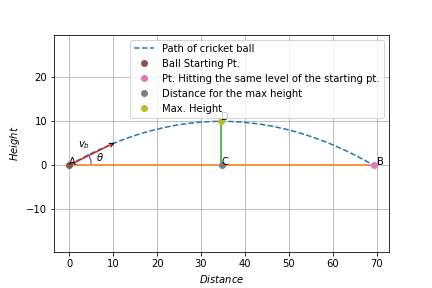
\includegraphics[width= \columnwidth]{assignment5.png}
    \caption{} \label{fig:1}
\end{figure}
\item[b)]The ball will return to the same level when vertical component of the distance function is equal to zero.
\begin{align}
    -4.9{t^2}+14t &= 0\\
    t &= 2.8572 s
\end{align}
Thus the time taken by the ball to return to the same level = 2.8572 $s$

\item[c)]Consider,
\begin{align}
    \vec{s}(2.8572) &=\myvec{69.283\\0}
\end{align}
Thus the distance from the thrower to the point where the ball returns to the same level = 69.283 $m$

\end{enumerate}




\end{document}
